\documentclass[journal]{IEEEtran}
\usepackage[utf8]{inputenc}
\usepackage{amsmath}
\usepackage{amsfonts}
\usepackage{amssymb}
\usepackage{graphicx}
\usepackage[left=2cm,right=2cm,top=2cm,bottom=2cm]{geometry}
\usepackage[export]{adjustbox}
\usepackage{subfigure,color,amsmath,amssymb,amsfonts}
\usepackage{url,graphicx,subfigure}

% Some handy Latin commands
\newcommand{\etal}{\textit{et al}.}
\newcommand{\ie}{\textit{i}.\textit{e}.,}
\newcommand{\eg}{\textit{e}.\textit{g}.}

\begin{document}
\title{Implementation of MRRC Alamouti Algorithm in a Rayleigh Fading Channel}
\author{Alon S. Levin\thanks{The Cooper Union, Department of Electrical Engineering}\\Wireless Communications\\ECE-408 --- Spring 2020}
\maketitle

\begin{abstract}
In 1998, Siavash M. Alamouti presented a new technique for increasing the diversity of a communications system utilizing two transmit antennas and one (or more) receive antennas, and compared this technique to the maximal-ratio receive combining (MRRC) technique that utilized a single transmit antenna and multiple receive antennas. This paper presents implementations of the two systems discussed by Alamouti, and presents the resulting bit error rates (BER) obtained when simulating these systems across a Rayleigh fading channel with additive white Gaussian noise (AWGN) of varying SNR.
\end{abstract}

\begin{IEEEkeywords}
Space-time coding, transmitter diversity, Alamouti algorithm, MRRC
\end{IEEEkeywords}

%%%%%%%%%%%%%%%%%%% Introductions %%%%%%%%%%%%%%%%%%
\section{Introduction}\label{sec:intro}
This project consisted of three main steps:
\begin{enumerate}
\item Simulating a Rayleigh fading channel using Smith's simulation methodology;
\item Implementing a communications link for 1 transmitter and $M$ receivers using the MRRC algorithm; and
\item Implementing a communications link for 2 transmitters and $M$ receivers using Alamouti's novel algorithm.
\end{enumerate}
To each of these tasks will be devoted an individual section in the remainder of this report, following which would be the results of these simulations and a discussion thereof.


\section{Rayleigh Fading Channel} \label{sec:channel}
A computer algorithm for modeling a multipath fading channel was published by J. I. Smith in 1975, which utilized  complex Gaussian noise source and a discretized spectrum model to generate a time-domain signal representing the channel. 

Rappaport breaks down the algorithm into the following steps:
\begin{enumerate}
\item Specify the number of frequency domain points ($N$) used to represent $\sqrt{S_{E}(f)}$ and the maximum Doppler frequency shift ($f_m$). The value used for $N$ is usually a power of 2. 
\item Compute the frequency spacing between adjacent spectral lines as $\Delta f = 2f_m / (N-1)$. This defines the time duration of a fading waveform, $T = 1/\Delta f$.
\item Generate complex Gaussian random variables for each of the $N/2$ positive frequency components of the noise source.
\item Construct the negative frequency components of the noise source by conjugating positive frequency values and assigning these at negative frequency values.
\item Multiply the in-phase and quadrature noise sources by the fading spectrum $\sqrt{S_{E}(f)}$.
\item Perform an IFFT on the resulting frequency domain signals from the in-phase and quadrature arms to get two N-length time series, and add the squares of each signal point in time to create an N-point time series.
\item  Take the square root of the sum obtained in step 6 to obtain an $N$~-point time series of a simulated Rayleigh fading signal with the proper Doppler spread and time correlation.
\end{enumerate}

This algorithm is represented graphically in Fig.~\ref{fig:SmithAlgorithm}. The spectrum $S_{E}(f)$ is defined by Clarke's model as
\begin{equation}
S_{E}(f) = \frac{1.5}{\pi f_m \sqrt{1 - \left(\frac{f - f_c}{f_m}\right)^2}}
\end{equation}

\begin{figure}
    \centering
    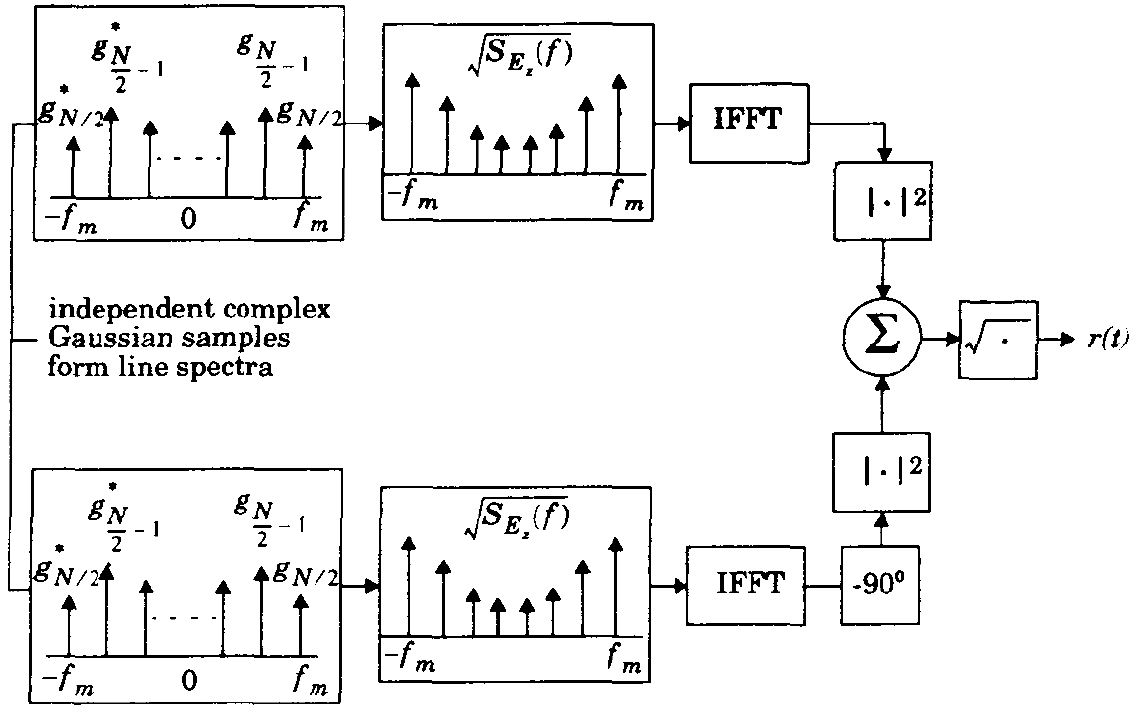
\includegraphics[width = 0.45\textwidth]{SmithAlgorithm}
    \caption{Block diagram of Smith's algorithm for simulating a Rayleigh fading channel. Recreated from Rappaport, Fig. 5.25.}
    \label{fig:SmithAlgorithm}
\end{figure}

\subsection{Implementation Details}
The channel was simulated at baseband, so $f_c$ was taken to be 0. To estimate the endpoints of the spectrum, at which $f - f_c = f = \pm f_m$, the value of $S_E(f = f_m)$ was estimated as $S_E(0.9999f_m)$; this does not faithfully follow Smith's original algorithm, which requires calculating the slope at the previous frequency sample and extending it.

\section{MRRC Implementation} \label{sec:MRRC}
The basic scheme for two-receiver MRRC is shown in Fig.~\ref{fig:MRRC_block}. However, in this section we will explore general solutions for $M$ receivers.

\begin{figure}
    \centering
    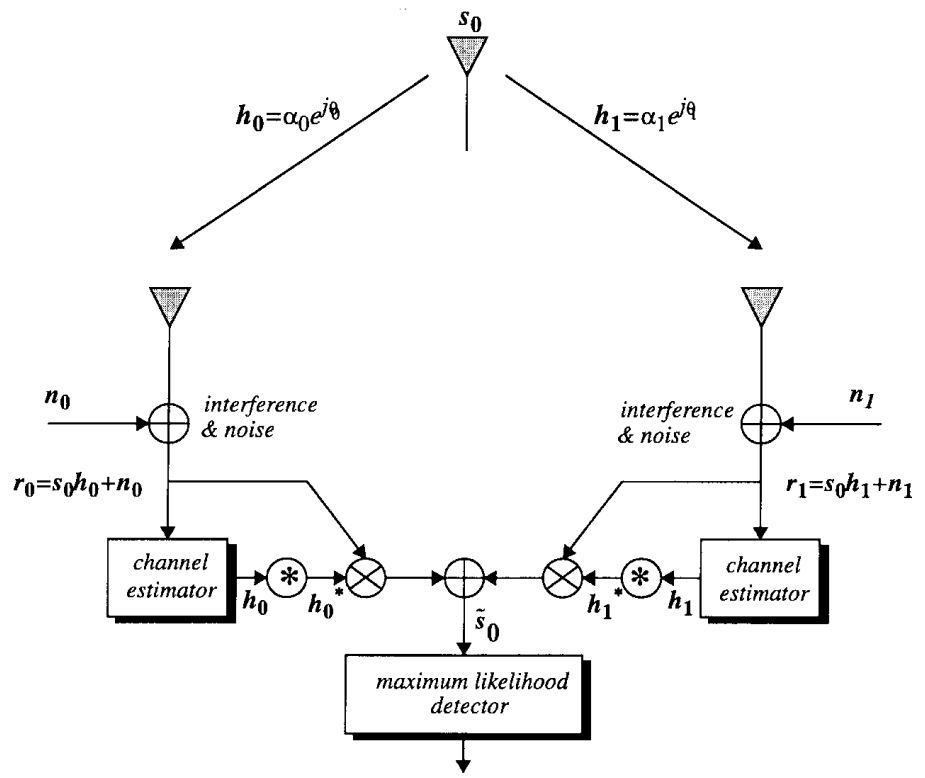
\includegraphics[width = 0.45\textwidth]{MRRC-2}
    \caption{Block diagram of the standard MRRC scheme, using two receivers. Recreated from the Alamouti paper.}
    \label{fig:MRRC_block}
\end{figure}

A single signal $\pmb{s_0}$ is transmitted at all times to $M$ separate receivers, thereby obtaining $M$ different received signals $\pmb{r_i}$ caused by two different channels $\pmb{h_i}$:
\begin{equation}
\pmb{r_i} = \pmb{h_i s_i} + \pmb{n_i}, \; i = 0,1,2,\ldots,M-1
\end{equation}
where $\pmb{n}$ represents additive white Gaussian noise (AWGN).

Assuming that all channels are known (obtained through channel estimation techniques not discussed here), an estimated signal $\pmb{\tilde{s_0}}$ can be easily obtained by inverting the channels:
\begin{equation}
\pmb{\tilde{s_0}} = \sum_{i=0}^{M-1} \pmb{h_i^* r_i}
\end{equation}

A maximum-likelihood (ML) estimator is used to determine which symbol was originally sent; for signals with equal energy constellations (i.e., PSK symbols), the decision rule simplifies to choosing $\pmb{s_i}$ if and only if
\begin{equation} \label{eq:ML_est}
d^2(\pmb{\tilde{s_0}}, \pmb{s_i}) \leq d^2(\pmb{\tilde{s_0}}, \pmb{s_k}), \; \forall \pmb{i}\neq\pmb{k},
\end{equation}
where $d^2(\pmb{x}, \pmb{y})$ represents the Euclidean distance between signals $\pmb{x}$ and $\pmb{y}$:
\begin{equation} \label{eq:euclid}
d^2(\pmb{x}, \pmb{y}) = (\pmb{x} - \pmb{y})(\pmb{x^*} - \pmb{y^*}).
\end{equation}

\section{Alamouti's Algorithm Implementation} \label{sec:alamouti}
Alamouti proposed a new diversity scheme which utilizes two transmitters to $M$ receivers across $N = 2M$ channels. Two such systems are presented in Fig.~\ref{fig:Alamouti_1_block} and Fig.~\ref{fig:Alamouti_2_block} for 1-receiver and 2-receiver systems. Here we will explore the general case for M receivers.
\begin{figure}
    \centering
    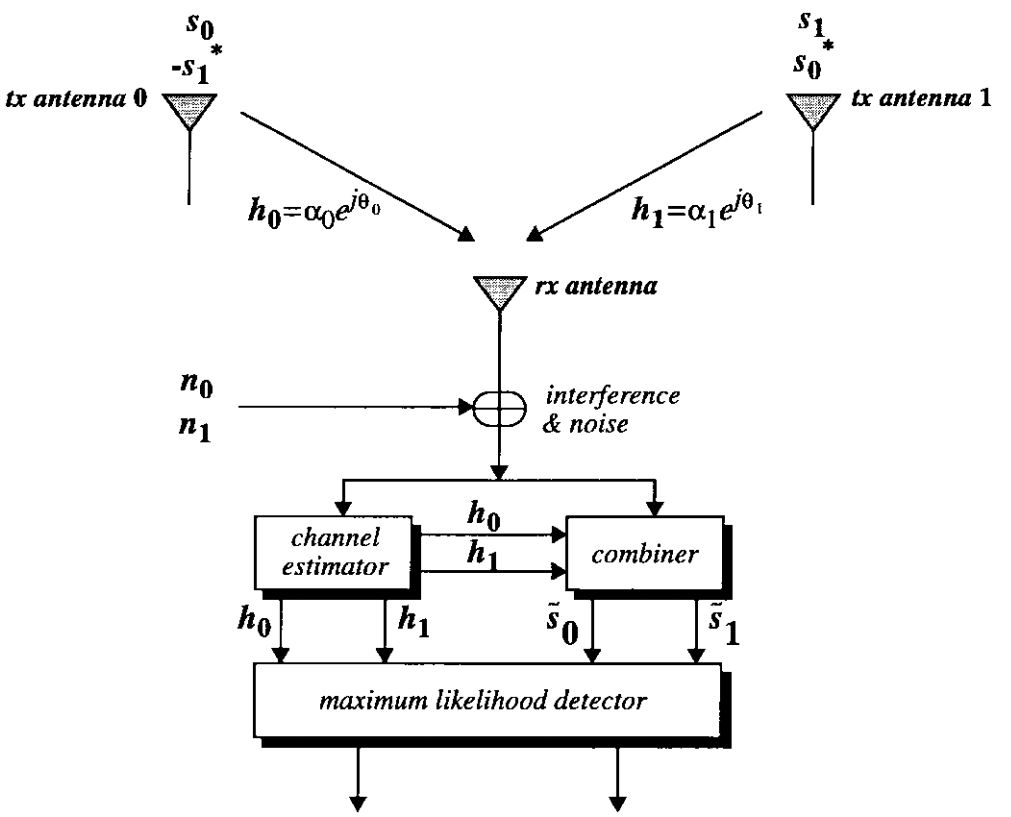
\includegraphics[width = 0.45\textwidth]{Alamouti-1}
    \caption{Block diagram of Alamouti's proposed diversity scheme, using a single receiver. Recreated from the Alamouti paper.}
    \label{fig:Alamouti_1_block}
\end{figure}
\begin{figure}
    \centering
    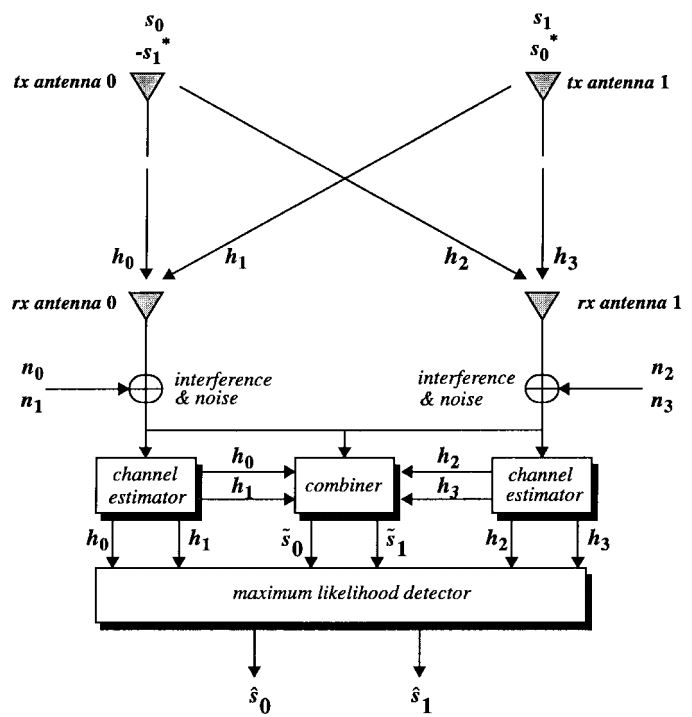
\includegraphics[width = 0.45\textwidth]{Alamouti-2}
    \caption{Block diagram of Alamouti's proposed diversity scheme, using two receivers. Recreated from the Alamouti paper.}
    \label{fig:Alamouti_2_block}
\end{figure}

Two signals $\pmb{s_0}$ and $\pmb{s_1}$ are transmitted from the two antennas over two time slots as per Tab.~\ref{tab:tx_seq}.

\begin{table}
\begin{center}
\begin{tabular}{c|c|c|}
\hline
 & antenna 0 & antenna 1 \\ 
\hline 
time $t$ & $\pmb{s_0}$ & $\pmb{s_1}$ \\ 
\hline 
time $t + T$ & $\pmb{-s_1^*}$ & $\pmb{s_0^*}$ \\
\hline
\end{tabular} 
\end{center}
\caption{The encoding and transmission sequence for an M-branch transmit diversity scheme. \label{tab:tx_seq}}
\end{table}

At times $t$ and $t + T$, receiver antenna $i$ receives the following signal:
\begin{eqnarray}
\pmb{r_i}(t) &=& \pmb{h_{2i} s_0} + \pmb{h_{2i + 1} s_0} + \pmb{n_i} \nonumber \\
\pmb{r_i}(t+T) &=& -\pmb{h_{2i} s_1^*} + \pmb{h_{2i + 1} s_0^*} + \pmb{n_i} \nonumber \\
i &=& 0,1,2,\ldots , M-1
\end{eqnarray}

The estimated symbols are obtained by the following combining scheme:
\begin{eqnarray}
\pmb{\tilde{s_0}} &=& \sum^{M-1}_{i=0} \left( \pmb{h_{2i}^* r_{i}}(t) + \pmb{h_{2i+1} r_{i}^*}(t+T) \right) \nonumber \\
\pmb{\tilde{s_1}} &=& \sum^{M-1}_{i=0} \left( \pmb{h_{2i+1}^* r_{i}}(t) - \pmb{h_{2i} r_{i}^*}(t+T) \right)
\end{eqnarray}
after which the same ML estimator from Eq.~\ref{eq:ML_est} and Eq.~\ref{eq:euclid} is used to determine which symbol was originally transmitted.

\section{Results \& Discussion}
Five different diversity schemes were simulated through a fading Rayleigh channel with $f_m = 1~\text{Hz}$. These five schemes were, in order:
\begin{enumerate}
\item No diversity (1 Tx, 1 Rx);
\item MRRC (1 Tx, 2 Rx);
\item MRRC (1 Tx, 4 Rx);
\item Alamouti's new scheme (2 Tx, 1 Rx); and
\item Alamouti's new scheme (2 Tx, 2 Rx).
\end{enumerate}

Each transmission consisted of 1,000 BPSK symbols; 100 iterations of the simulation were performed with each scheme at each SNR value, with new transmissions and channels generated each time. 16 different SNR values were tested, equally spaced between 0 dB and 50 dB. The results are shown in Fig.~\ref{fig:BER_mine}.
\begin{figure}
    \centering
    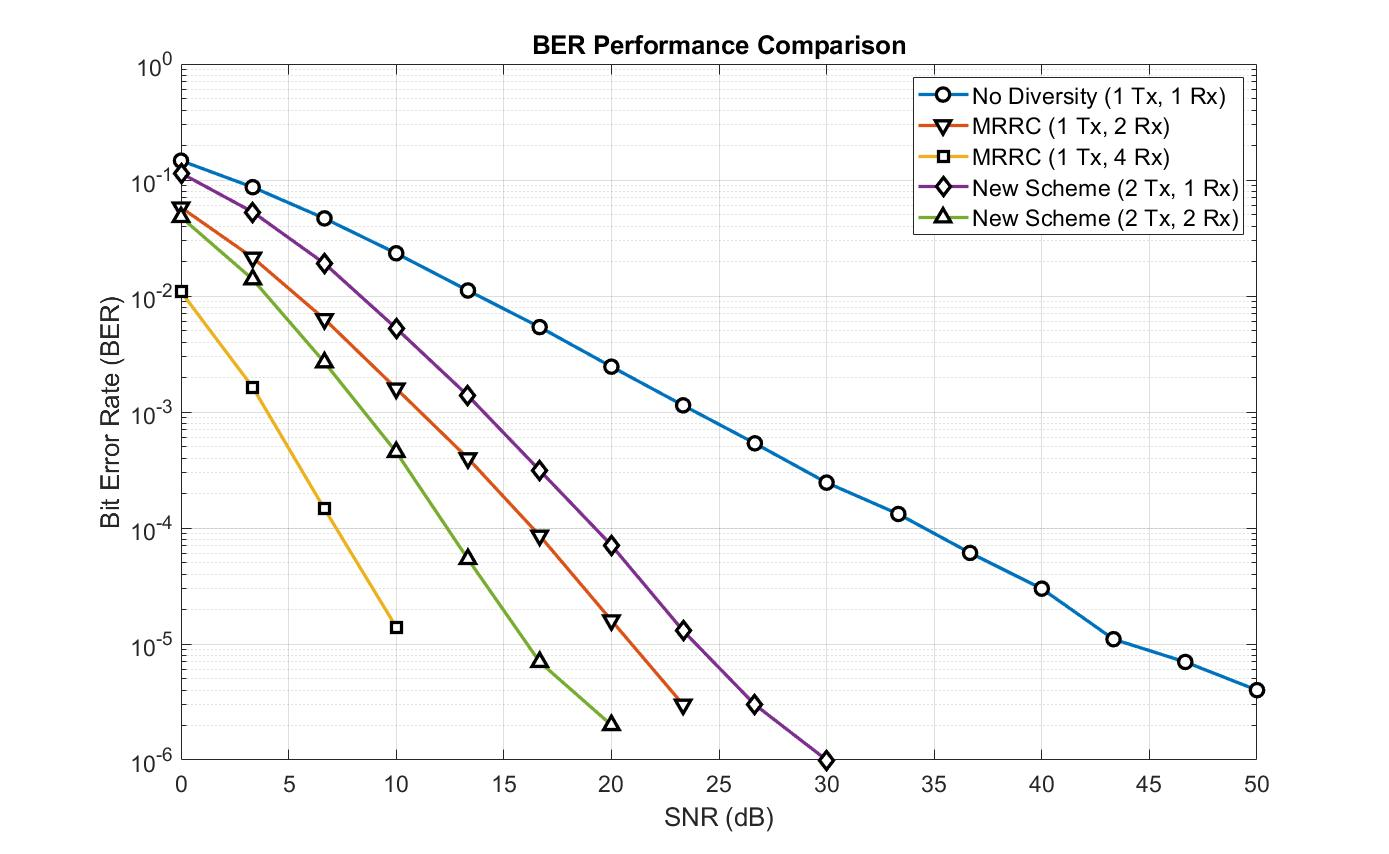
\includegraphics[width = 0.45\textwidth]{BER}
    \caption{Simulated results showing the performance of each of the five schemes tested.}
    \label{fig:BER_mine}
\end{figure}

These empirical results align nearly perfectly with Alamouti's simulation results, recreated from his paper in Fig.~\ref{fig:BER_alamouti}. Furthermore, when double transmission power was used to account for the power halving due to transmit antenna doubling, the MRRC-2Rx \& Alamouti-1Rx and MRRC-4Rx \& Alamouti-2Rx curves overlap almost exactly --- just as predicted by Alamouti in his paper. This indicates the fundamental equivalence between the standard $2M$-branch MRRC scheme and $M$-branch space-time diversity scheme, given equal antenna transmission power.
\begin{figure}
    \centering
    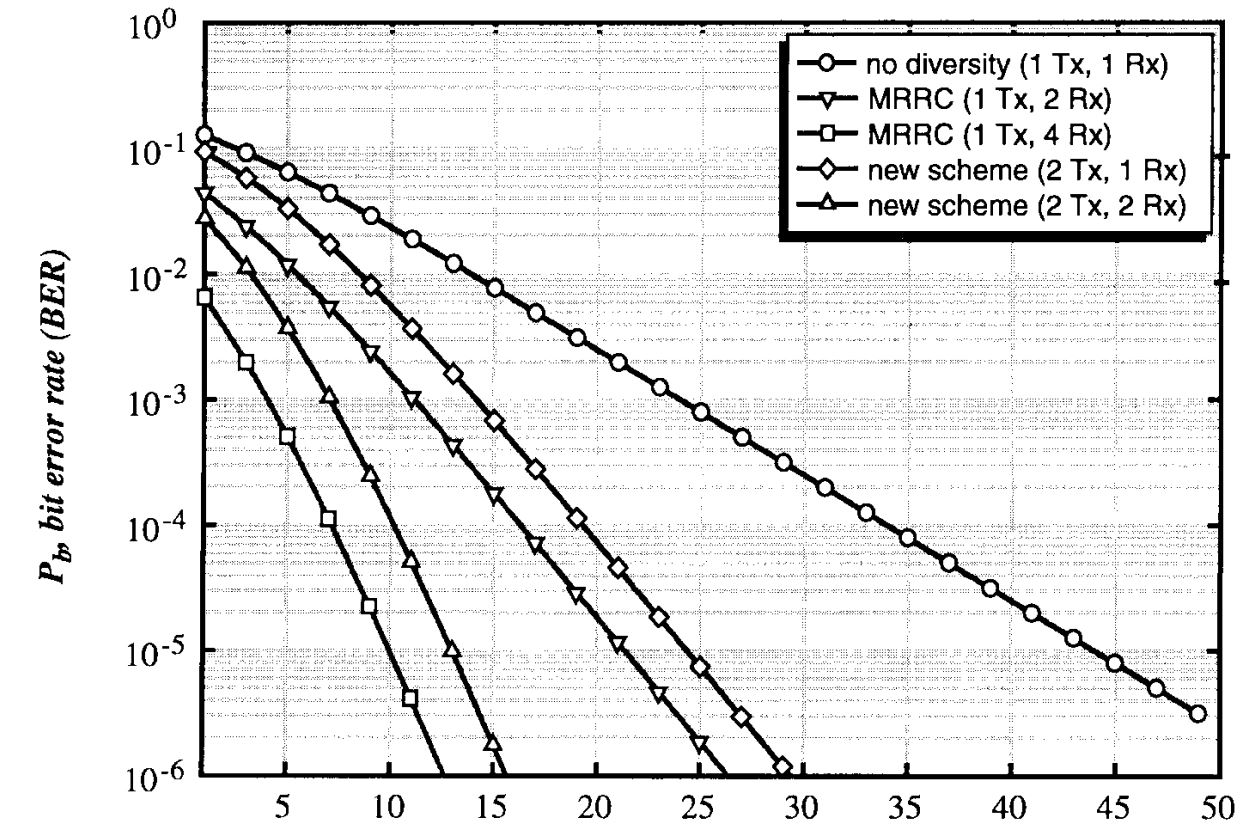
\includegraphics[width = 0.45\textwidth]{BER_alamouti}
    \caption{Results, as presented by Alamouti.}
    \label{fig:BER_alamouti}
\end{figure}

In general, Alamouti's space-time diversity scheme does not require exactly two antennas. Alamouti defined the simplest space-time block code, denoted by the coding matrix
\begin{equation}
C_2 = \begin{bmatrix}
c_1 & c_2 \\
-c_2^* & c_1^*
\end{bmatrix},
\end{equation}
in which the columns represent symbol time slots and the rows represent each transmit antenna's signal. Since publication, new techniques were created that would allow for a greater number of transmit antennas, albeit at the cost of a lower data rate to preserve orthogonality.


%%%%%%%%%%%%%%%%%%% Bibliography %%%%%%%%%%%%%%%%%%%
\bibliographystyle{unsrt}
%% To reload citations:
%% F6 --> F11 --> F6 --> F6 --> F7
\bibliography{Bibliography} %filename (no .bib)

\end{document}